% Устанавливаем размер шрифта в 14 пунктов.
% Рекомендованный размер шрифта по ГОСТ 7.32-2017 ---
% не менее 12 пунктов [1, §́ 6.1.1].
\documentclass[14pt,russian]{extarticle}

\usepackage{amsmath}

\usepackage{array}
\usepackage{graphicx}

\usepackage[math]{cellspace}
\cellspacetoplimit 4pt
\cellspacebottomlimit 4pt

% Настройка формат страниц и величины полей согласно [1, § 6.1.1].
\usepackage[
	a4paper,
	bindingoffset=0pt,
	left=30mm,
	right=15mm,
	top=20mm,
	bottom=20mm,
	footskip=0mm,
	includeheadfoot,
	]{geometry}

% Просим LaTeX попытаться избежать строк- «сирот» и «вдов».
\usepackage[all]{nowidow}

% Поддержка кириллицы и кодировки UTF-8.
\usepackage[T1,T2A]{fontenc}
\usepackage[utf8]{inputenc}
\usepackage[english,main=russian]{babel}

% Поддержка вставки изображений в документ.
\usepackage{graphicx}
\graphicspath{{./img/}}

% Плавающее положение изображений в документе.
\usepackage{float}

% Из ГОСТ.32-2017: «Иллюстрации при необходимости могут иметь наименование и
% пояснительные данные (подрисуночный текст). Слово "Рисунок", его номер и через
% тире наименование помещают после пояснительных данных и располагают в центре
% под рисунком без точки в конце» [1, 6.5.7].
%
% TODO: заменить en dash (короткое тире) на em dash (тире).
\usepackage[figurename=Рисунок,labelsep=endash]{caption}
% TODO
% 6.6.3 Наименование таблицы, при ее* наличии, должно отражать ее содержание, быть
% точным, кратким. Наименование следует помещать над таблицей слева, без абзацного
% отступа в следующем формате: Таблица Номер таблицы - Наименование таблицы.
% Наименование таблицы приводят с прописной буквы без точки в конце.
\captionsetup[table]{singlelinecheck=off}

% Из ГОСТ.32-2017: «Допускается нумеровать иллюстрации в пределах раздела
% отчета. В этом случае номер иллюстрации состоит из номера раздела и
% порядкового номера иллюстрации, разделенных точкой: Рисунок 2.1.» [1, 6.5.6].
\renewcommand{\thefigure}{\arabic{section}.\arabic{figure}}

% Поддержка автоматических переносов слов.
\usepackage{hyphenat}

% Из ГОСТ 7.32-2017: "Страницы отчета следует нумеровать арабским
% цифрами, соблюдая сквозную нумерацию по всему тексту отчета,
% включая приложения" [1, § 6.3.1].
\pagenumbering{arabic}

% Рекомендуемый по ГОСТ 7.32-2017 тип шрифта для основного текста отчета - Times
% New Roman [1, § 6.1.1].
%
% Способ задания шрифта Times New Roman с поддержкой кириллицы подсмотрен в
% источнике [2].
\usepackage{tempora}

% Полуторный интервал рекомендован [1, § 6.1.1].
\usepackage{setspace}
\onehalfspacing

% ГОСТ 7.32-2017: "Абзацный отступ должен быть одинаковым по всему
% тексту отчета и равен 1,25 см." [1, § 6.1.1].
\setlength{\parindent}{1.25cm}

% LaTeX по-умолчанию выравнивает текст по ширине, что и требуется по
% ГОСТ.32-2017.
% TODO: привести ссылку на требование.

% Формат заголовков: размер шрифта, интерлиньяж и расстояние между
% порядковым номером и сами заголовком. Последнее берется равным абзацному
% отступу (1,25 см).
%
% TODO: найти, какие требования к оформлению заголовков предъявляет [1].
\usepackage{titlesec}
\titleformat{\section}{\normalfont\fontsize{18pt}{\baselineskip}\bfseries}{\thesection}{1.25cm}{}
\titleformat{\subsection}{\normalfont\fontsize{16pt}{\baselineskip}\bfseries}{\thesubsection}{1.25cm}{}
\titleformat{\subsubsection}{\normalfont\fontsize{14pt}{\baselineskip}\bfseries}{\thesubsubsection}{1.25cm}{}

% Задаем тире как символ для элементов в списках.
% TODO: найти, какие требования предъявляет [1] к оформлению списков.
\renewcommand{\labelitemi}{---}

% Поддержка библиографического списока по ГОСТ 7.0.5-2008.
% https://github.com/odomanov/biblatex-gost
\usepackage{csquotes}
\usepackage[backend=biber,style=gost-numeric,sorting=none]{biblatex}
\addbibresource{bibliography.bib}

% Из ГОСТ.32-2017: «Заголовки структурных элементов следует располагать в
% середине строки без точки в конце, прописными буквами, не подчеркивая. Каждый
% структурный элемент и каждый раздел основной части отчета начинают с новой
% страницы» [1, § 6.2.1].
\newcommand*\gostStructureElement[1]{
	\clearpage
	\section*{\centerline{\MakeUppercase{#1}}}
	\addcontentsline{toc}{section}{\MakeUppercase{#1}}
}

% Из ГОСТ.32-2017: «Использование курсива допускается для обозначения объектов
% (биология, геология, медицина, нанотехнологии, генная инженерия и др.) и
% написания терминов (например, in vivo, in vitro) и иных объектов и терминов на
% латыни» [1, § 6.1.1].
\newcommand*\obj[1]{\textit{#1}}
\newcommand*\term[1]{\textit{#1}}

% То же, что и выше для содержания.
\usepackage{etoc}
\etocsettocstyle{\centerline{\MakeUppercase{\textbf{Содержание}}}}

% TODO https://tex.stackexchange.com/questions/410250/understanding-line-height-line-spacing-baselineskip-in-latex
\usepackage{fix-cm}

%-------------------------------------------------------------------------------
%
% НАЧАЛО ДОКУМЕНТА
%
%-------------------------------------------------------------------------------

\title{Выпускная квалификационная работа "Разработка компилятора языка C для
образовательных целей"}
\author{Нефедов Д. В.}
\date{Октябрь 2021}

\begin{document}

% Из ГОСТ 7.32-2017: "Титульный лист включают в общую нумерацию страниц отчета.
% Номер страницы на титульном листе не проставляют" [1, § 6.3.2].
\begin{titlepage}
	\begin{center}
		\singlespacing

		Министерство образования и науки Российской Федерации

		\MakeUppercase{Федеральное государственное бюджетное
		образовательное учреждение высшего образования Саратовский
		Государственный Технический Университет имени Гагарина Ю.А.}

		(СГТУ им. Гагарина Ю.А.)

		\bigskip
		\bigskip

		Кафедра ``Прикладные информационные технологии''

		\bigskip
		\bigskip
		\bigskip
		\bigskip
		\bigskip
		\bigskip
		\bigskip
		\bigskip

		% Вид документа
		\singlespacing

		ОТЧЕТ О

		НАУЧНО-ИССЛЕДОВАТЕЛЬСКОЙ РАБОТЕ

		\MakeUppercase{Лабораторная работа по выбору и установке
		операционной системы}

		\onehalfspacing
	
		(промежуточный, этап 1)

		\bigskip
		\bigskip

		Программные и аппаратные технологии умного города
	\end{center}

	\bigskip
	\bigskip

	\begin{flushleft}
		\singlespacing

		Исполнитель НИР,

		студент б1-ПИНФ-41 \_\_\_\_\_\_\_\_\_\_ Нефедов Д.В.

		\singlespacing

		Руководитель НИР,

		канд. техн. наук, доц. \_\_\_\_\_\_\_\_\_\_ Федукин А.Ю

		% \begingroup
		% 	\fontsize{12pt}{1}\selectfont
		% 	\hspace{11em} подпись, дата
		% \endgroup
	\end{flushleft}

	\vfill
	\centerline{Саратов 2021}
\end{titlepage}

\newgeometry{
	bindingoffset=0pt,
	left=30mm,
	right=15mm,
	top=20mm,
	bottom=20mm,
	footskip=20mm,
	includeheadfoot}

% Содержание является обязательным структурным элементом
% отчета о НИР согласно [1, § 4].
\clearpage
\tableofcontents

\gostStructureElement{Введение}

Компиляторы --- это критические важные программные системы. Без компиляторов
было бы невозможно представить себе сегодняшний мир, ведь написание любой
сколько-нибудь сложной компьютерной программы требует использования языков
программирования высокого уровня.

Такие языки избавляют программистов от трудоемкости и сложности написания
программного кода на языках ассемблера, которые требуют от программиста
детального знания устройства ISA конкретного процессора \cite{keith1}. Языки программирования
высокого уровня позволяют абстрагироваться от деталей конкретной архитектуры и
сфокусироваться на решение задачи, которая стоит перед разрабатываемой
компьютерной программой.

Кроме того, использование ЯП высокого уровня позволяет допускать гораздо меньше
ошибок по сравнению с языками ассемблера. В предотвращении ошибок помогает
встроенные в компилятор проверки синтаксиса и семантики. Это особенно актуально
для строго типизированных языков программирования.

Зачастую компиляторы генерируют гораздо более эффективный ассемблерный код, чем
смог бы написать программист \cite{randall1}. Это не удивительно, ведь написание эффективного
ассемблерного кода требует от программиста глубочайшего понимания архитектуры
процессора, под который пишется программа, внимание к мельчайшим деталям,
стоимость выполнения каждой инструкций в микрооперациях и многое другое. Хорошо
известного, что человеку тяжело работать с большим объемом чисел и просчитывать
мельчайшие детали. Для такой работы и были придуманы компьютеры, а значит именно
у них получится генерировать более эффективный низкоуровневый код, чем мог бы
написать программист.

К сожалению, компиляторы сами по себе являются сложнейшими компьютерными
программами, которые состоят из десятков модулей, требуют знания в самых
различных областях информатики \cite{Aho1}. Оптимизирующие компиляторы требуют особых
навыков, так как разработка алгоритмов оптимизации находится на рубежах науки и
людей, которые могли бы разработать и реализовать определенный алгоритм
оптимизации в компиляторе не так уж и много.

Более того, так как компиляторы --- это огромные компьютерные программы, состоящие
из десятков миллионов строк кода, то столь же мало людей, которые разбираются в
кодовой базе, причем в основном каждый разработчик разбирается только в своем
модуле, не понимая ничего, либо крайне мало о других модулях компилятора.

Для примера, в компиляторе GCC по состоянию на 5 января 2015 года было чуть
более 14,5 миллионов строк кода \cite{gcc1}. Что интересно, код компилятора GCC
был настолько сложен, что в нем существовал модуль под названием ``reload'',
функционал которого до сих пор не до конца понятен самим разработчикам GCC
\cite{gcc2}.

Чрезвычайная сложность компиляторов представляет большую проблему для студентов:
нет простых и понятных примеров, на которые можно было бы взглянуть. Учебники по
разработке компиляторов порой слишком обстоятельны и формальны, что усложняет
усвоение информации --- достаточно вспомнить классическую ``Книгу дракона''.

Одним из возможных решений данной проблемы является создание простого и
понятного компилятора, в исходном коде и архитектуре которого легко разобраться.
Наша АИС направлена на решение этой проблемы.

\clearpage
\section{Описание предметной области}

\subsection{Цель курсовой работы}

Целью курсовой работы являются закрепление теоретических знаний, получение
практических навыков и новых знаний в области проектирования информационных
систем.

Цель работы достигается в результате участия в решении практических задач и
проблем, возникающих при разработке информационной системы компилятора языка C.

\subsection{Словесное описание предметной области}

Информационная система компилятора языка C предназначена для образовательных
целей и предназначена для обучения студентов и прочих желающих внутреннему
устройству и построению в частности компиляторов, а в общем случае ---
программ-трансляторов с одного языка программирования в другой.

Система ориентирована в первую очередь на студентов технических направлений.
Техническое задание по разработанной системе находится в Приложении А.

\clearpage
\section{Уточнение описания предметной области}

\subsection{IDEF0}

IDEF0 является методологией функционального моделирования. Она используется для
создания функциональной модели, которая отображает структуру и функции системы,
а также потоки информации и материальных объектов, связывающих эти функции.
Компонентами синтаксиса IDEF0 являются блоки, стрелки, диаграммы и правила
\cite{defense1}.

Диаграмма IDEF0 состоит из \obj{блоков} и \obj{стрелок}, направление которых
заданы правила. Блоки изображаются в виде прямоугольников и содержат в себе
описание той функции, которую они представляют, и номер. Номер блока должен быть
расположен в правом нижнем углу.

К каждому блоку должно вести несколько стрелок, такие как:

\begin{itemize}
	\item \obj{левые стрелки} (направлены в блок) обозначают информацию или
		продукты, которую функция получает на входе;

	\item \obj{правые стрелки} (направлены из блока) обозначают информацию
		или продукты, которую функция дает на выходе;

	\item \obj{верхние стрелки} (направлены в блок) обозначают документы,
		которые регламентируют работы системы;

	\item \obj{нижние левые стрелки} (направлены в блок) обозначают
		механизмы, которые влияют на работу нашей системы;

	\item \obj{нижние правые стрелки} (направлены из блока) обозначают
		обращение к дополнительной информационной системе, которая
		существует совершенно отдельно от нашей и которая необходима для
		осуществления процесса или функции. Может как присутствовать на
		схеме, так и нет.
\end{itemize}

\begin{figure}[H]
	\centering
	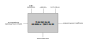
\includegraphics[width=\textwidth,clip=true]{img/IDEF0-1.png}
	\caption{Комплексная диаграмма IDEF0}
\end{figure}

\begin{figure}[H]
	\centering
	
\includegraphics[width=\textwidth,clip=true]{img/IDEF0-2.png}
	\caption{Декомпозиция комплексной диаграммы IDEF0}
\end{figure}

\subsection{IDEF3}

Методология IDEF3 –-- это методология описания процессов. В отличие от IDEF0 она
рассматривает последовательность выполнения задач, а также причинно-следственные
связи между ними \cite{idef3}. Диаграммы IDEF3 состоят из блоков, описывающих функции,
стрелок-связей и перекрёстков, которые показывают, как именно выполняются
процессы.

\obj{Блок} (функциональный элемент) представляет собой прямоугольник, разделенный на
три другие прямоугольника: один большой наверху и два маленьких друг рядом с
другом внизу. В верхнем прямоугольнике содержится имя функции, в нижнем левом
номер его выполнения, в нижнем правом, при необходимости, находится ссылка на
другую функцию. Связи бывают простыми, относительными и связями с условием.

Перекрёстки подразделяются на следующие типы: \obj{И}, \obj{ИЛИ},
\obj{синхронное И}, \obj{синхронное ИЛИ}, а также \obj{исключающее ИЛИ}.

\begin{figure}[H]
	\centering
	
\includegraphics[width=\textwidth,clip=true]{img/IDEF3.png}
	\caption{IDEF3 диаграмма}
\end{figure}

\subsection{DFD}

\term{Диаграммы потоков данных} (англ. \term{DFD}) –-- это способ представления
процессов обработки информации. Они показывают, как информация перемещается из
одной функции к другой. Подобное представление потока данных отражает движение
объектов, их хранение и распространение.

DFD состоит из следующих компонентов: внешняя сущность, процесс, поток данных и
хранилище данных \cite{dfd}. Внешняя сущность представляет собой источник или приёмник
информации и изображается прямоугольником с прямыми углами. Процессы в DFD – это
функции системы, преобразующие входы и выходы, которые изображаются как
прямоугольники со скругленными углами. Потоки данных изображаются стрелками.
Если стрелка соединяет какую-либо функцию с хранилищем данных, то на ней должно
быть отображено имя, отражающее содержание данного потока. Хранилище данных
является прообразом базы данных и изображается как прямоугольник без правой
стороны.

\begin{figure}[H]
	\centering
	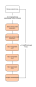
\includegraphics[height=0.8\textwidth,keepaspectratio,clip=true]{img/DFD.png}
	\caption{DFD диаграмма}
\end{figure}

\subsection{UML}

\term{UML} является унифицированным языком моделирования, объекты в котором это
упрощенное представление предметов окружающего нас мира \cite{hunt}. Его используют при
разработке ПО для моделирования бизнес-процессов, системного проектирования и
отображения организационных структур \cite{fowler}. UML диаграммы подразделяются на два типа:
структурные и поведенческие.

\subsubsection{Диаграмма пакетов}

\term{Диаграмма пакетов} --- это структурная диаграмма UML, которая показывает
структуру проектируемой системы на уровне пакетов \cite{martin}. Обычно на диаграмме
изображаются следующие элементы: пакет, пакетированный элемент, зависимость,
импортируемый элемент, импорт пакета, объединение пакета.

\begin{figure}[H]
	\centering
	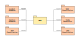
\includegraphics[width=\textwidth,clip=true]{img/UML-package.png}
	\caption{Диаграмма пакетов UML}
\end{figure}

\subsubsection{Диаграмма компонентов}

\term{Диаграмма компонентов} показывает компоненты, предоставляемые и требуемые
интерфейсы, порты и отношения между ними \cite{buch}. Этот тип диаграмм используется в
компонентно-ориентированной разработке для описания систем с
сервисно-ориентированной архитектурой \cite{douglass}.

Компонентно-ориентированная разработка основана на предположения, что ранее
сконструированные компоненты могут быть переиспользованы или, при необходимости,
заменены на некие ``эквивалентные'' или ``совместимые'' компоненты.

\begin{figure}[H]
	\centering
	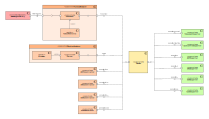
\includegraphics[width=\textwidth,clip=true]{img/UML-components.png}
	\caption{Диаграмма компонентов UML}
\end{figure}

\subsubsection{Диаграмма потока информации}

\term{Диаграмма потока информации} --- это поведенческая диаграмма UML, которая
показывает обмен информацией между сущностями системы на высоком уровне
абстракции. Потоки информации могут быть полезны для описания циркуляции
информации через систему через представление аспектов модели, которые еще не
полностью специфицированы или недостаточно детализированы.

Потоки информации не показывают природу информации, механизмы передачи, порядок
обмена или какие-либо контрольные условия \cite{penker}. Единицы информации могут быть
использованы для представления информации, которая протекает через систему
вместе с информационными потоками еще прежде, чем их реализация будет
проработана.

\begin{figure}[H]
	\centering
	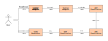
\includegraphics[scale=1.35,clip=true]{img/UML-information-flow.png}
	\caption{Диаграмма потока информации UML}
\end{figure}

\clearpage
\section{Выбор средств разработки}

Так как для компилятора требуется возможность скомпилировать самого себя, то
выбор реализации языка становится очевиден --- это язык C стандарта ISO/IEC
9899:1999.

Кроме того, из соображений минимизации зависимостей для более полного понимания
всего процесса компиляции единственной зависимостью компилятора будет
использование функций GNU C Library, реализующих POSIX-совместимые регулярные
выражения, которые не входят в используемый стандарт языка.

В рамках реализации компилятора не ставится задача реализации собственного
движка регулярных выражений, так как это довольно простая математическая модель
(регулярные языки), разработка которых лишь усложнит код компилятора, который мы
стараемся сделать максимально простым.

Для облегчения процесса сборки приложения в качестве средств систем сборки будет
использован такой инструмент как GNU Make.

В качестве компилятора может быть использован любой компилятор, который
поддерживает стандарт ISO/IEC 9899:1999. Более того, использование разных
компиляторов позволит убедится, что исходный код компилятора соответствует
используемому стандарту.

\clearpage
\section{Оценка стоимости работ}

Варианты использования описывают основные процедуры работы с системой, поэтому
путём их анализа можно определить сложность системы, а, значит, и затраты,
необходимые для её разработки. Во многих случаях исследование вариантов
использования проще, чем поиск функциональных точек, необходимых для работы
других методов оценивания затрат, таких как COCOMO II и Functional Points.

Сложность системы при этом определяется следующими факторами:

\begin{itemize}
	\item количество и сложность действующих лиц, участвующих в варианте использования;

	\item дополнительные требования, такие как многозадачность, безопасность и
		производительность;

	\item внешние факторы, такие как опыт членов команды разработчиков.
\end{itemize}

В качестве единицы сложности системы используется прецедентная точка (Use-Case
Point, UCP), количество таких точек для каждого варианта использования
определяется по формуле:

\begin{equation}
	\mathrm{UCP} = \mathrm{TCP} \times \mathrm{ECF} \times \mathrm{UUCP} \times \mathrm{PF}
\end{equation}

\begin{itemize}
	\item UCP – количество прецедентных точек;
	\item TCP – коэффициент технической сложности;
	\item ECF – коэффициент сложности взаимодействия с окружающей средой;
	\item PF – эффективность работы разработчиков;
	\item UUCP – количество нескорректированных прецедентных точек.
\end{itemize}

Значение UUCP определяется числом шагов, необходимых для выполнения варианта
использования, действующими лицами каждого варианта и общим количеством, и
сложностью вариантов использования рассматриваемом варианте использования 3
шага. Сложность варианта использования определяется в соответствие со следующими
правилами:

\begin{itemize}
	\item \textit{простой} (5 баллов) – предполагается простой пользовательский интерфейс
		и работа не более, чем с одной сущностью базы данных; количество шагов не
		превышает 3, а в реализации задействовано не более 5 классов;

	\item \textit{средней сложности} (10 баллов) – более сложный пользовательский
		интерфейс, работа с двумя или более сущностями базы данных; количество шагов
		составляет от 4 до 7, в реализации задействовано 5-10 классов;

	\item \textit{сложный} (15) – сложная обработка запросов пользователя, работа с тремя и
		более сущностями базы данных; количество шагов превышает 7, количество
		классов в реализации более 10.
\end{itemize}

Варианты использования:

\begin{itemize}
	\item \textit{простой}: выполнение лексического анализа единицы трансляции;
		выполнение синтаксического анализа, вывод диагностических сообщений о
		лексических ошибках в программе;

	\item \textit{средней}: построение AST по дереву разбора, вывод
		диагностических сообщений о синтаксических и лексических ошибках;

	\item \textit{сложный}: построение трехадресного кода, построение SSA, кодогенерация
		кода под целевую платформу.
\end{itemize}

\begin{equation}
	\mathrm{UUCW} = 3 \times 5 + 2 \times 10 + 3 \times 15 = 80
\end{equation}

Действующие лица также разделяются на три класса по следующим правилам:

\begin{itemize}
	\item \textit{простое действующее лицо} (1 балл) – сторонняя система, обращающаяся к
		нашей системе через программный интерфейс;

	\item \textit{действующее лицо средней сложности} (2 балла) – сторонняя система,
		обращающаяся к нашей по сети;

	\item \textit{сложное действующее лицо} (3 балла) – пользователь системы.
\end{itemize}

После этого подсчитывается количество действующих лиц в каждом классе,
количество умножается на соответствующие баллы. В результате получается
нескорректированный вес действующих лиц (UAW). В нашем варианте одно сложное
действующее лицо --- пользователь.

\begin{equation}
	\mathrm{UAW} = 1 \times 3 = 3.
\end{equation}

Значение UUCP вычисляется по формуле:

\begin{equation}
	\mathrm{UUCP} = \mathrm{UUCW} + \mathrm{UAW} = 80 + 3 = 83.
\end{equation}

Для вычисления TCF сначала каждому фактору присваивается вес в зависимости от
того, насколько сильно его влияние на систему (от 0 до 5). После этого
оценивается сложность, связанная с данным фактором (также от 0 до 5). Полученные
значения перемножаются, результаты складываются и получают значение PreTCF
(см. таблицу 1).

\begin{table}[H]
	\caption{Получение значения PreTCF}

	\resizebox{\textwidth}{!}{
		\begin{tabular}{|Sl|Sl|Sl|Sl|}
			\hline
				\multicolumn{1}{|c|}{Описание} &
				\multicolumn{1}{|c|}{Вес} &
				\multicolumn{1}{|c|}{Сложность} &
				\multicolumn{1}{|c|}{Вес × сложность} \\
			\hline
			Распределённая система & 0 & 5 & 0 \\
			Производительность & 0 & 4 & 0 \\
			Эффективность взаимодействия с пользователем & 5 & 3 & 15 \\
			Сложные алгоритмы обработки данных & 5 & 5 & 25 \\
			Возможность повторного использования & 5 & 5 & 25 \\
			Простота установки & 5 & 2 & 10 \\
			Простота использования & 5 & 3 & 15 \\
			Переносимость & 0 & 5 & 0 \\
			Простота модификации & 5 & 5 & 25 \\
			Многозадачность & 0 & 5 & 0 \\
			Безопасность & 0 & 4 & 0 \\
			Открытость для сторонних приложений & 5 & 4 & 20 \\
			Необходимость специальных навыков пользователей & 5 & 1 & 5 \\

			\hline
			PreTCF & \multicolumn{2}{|c|}{} & 144 \\
			\hline
		\end{tabular}
	}
\end{table}

Значение TCF вычисляется по формуле:

\begin{equation}
	\mathrm{TCF} = 0.6 + 0.01 \times \mathrm{PreTCF} = 0.6 + 1.44 = 2.04.
\end{equation}

Аналогичным образом вычисляется значение PreECF (см. таблицу 2).

\begin{table}[H]
	\caption{Получение значения PreECF}

	\resizebox{\textwidth}{!}{
		\begin{tabular}{|Sl|Sl|Sl|Sl|}
			\hline
				\multicolumn{1}{|c|}{Описание} &
				\multicolumn{1}{|c|}{Вес} &
				\multicolumn{1}{|c|}{Сложность} &
				\multicolumn{1}{|c|}{Вес × сложность} \\
			\hline
			Знакомство с UML & 1 & 1 & 1 \\
			Знакомство с предметной областью & 4 & 5 & 20 \\
			Знакомство с объектно-ориентированными технологиями & 3 & 2 & 6 \\
			Опыт ведущего аналитика & 2 & 3 & 6 \\
			Мотивация & 2 & 3 & 6 \\
			Постоянство требований & 1 & 1 & 1 \\
			Наличие совместителей & 0 & 3 & 0 \\
			Трудный язык программирования & 2 & 3 & 6 \\

			\hline
			PreECF & \multicolumn{2}{|c|}{} & 46 \\
			\hline
		\end{tabular}
	}
\end{table}

Значение ECF вычисляется по формуле:

\begin{equation}
	\mathrm{ECF} = 1.4 + (-0.03 \times \mathrm{PreECF}) = 1.4 - 1.38 = 0.02.
\end{equation}

Значение PF определяется как количество человеко-часов, необходимых для
реализации одного варианта использования. Данное значение определяется из опыта
выполнения предыдущих проектов. Если такой опыт отсутствует, то берётся число из
интервала от 15 до 30, обычно 20. Тогда:

\begin{equation}
	\mathrm{UCP} = 83 \times 2.04 \times 0.02 \times 20 \approx 67.60.
\end{equation}

Получили, что для реализации системы потребуется 67.60 человеко-часов.

\gostStructureElement{Заключение}

Таким образом, по итогу проделанной работы сделано следующее:

\begin{itemize}
	\item Изучена предметная область, проведен её анализ, определены цели и
		задачи системы;

	\item Сформулировано словесное описание разрабатываемой информационной
		системы;

	\item Изучены графические нотации методологий IDEF0, IDEF3, DFD и UML,
		их принципы построения, а также построены соответствующие
		модели, описывающие работу данной системы;

	\item Произведено оценивание стоимости создания информационной системы и
		выявлено, сколько потребуется человеко-часов для создания данной
		системы.
\end{itemize}

\clearpage
\printbibliography[heading=bibintoc,title=СПИСОК ИСПОЛЬЗОВАННЫХ ИСТОЧНИКОВ]

\gostStructureElement{Приложение А}

\end{document}

% 1. ГОСТ 7.32-2017. Система стандартов по информации, библиотечному и
%    издательскому делу. ОТЧЕТ О НАУЧНО-ИССЛЕДОВАТЕЛЬСКОЙ РАБОТЕ. Структура и
%    правила оформления.
% 2. How to set up Russian Cyrillic Times New Roman font in PdfLaTeX?.
%    <https://tex.stackexchange.com/q/405433/225663>.
